\documentclass[a4paper]{extarticle}
\usepackage[utf8]{inputenc}
\usepackage[english,russian]{babel}
\usepackage[T2A,T1]{fontenc}
\usepackage{amsmath}
\usepackage{amssymb}
\usepackage{tikz}
\usetikzlibrary{shapes,arrows,positioning, fit}
\usepackage[a4paper, top=20mm, left=30mm, right=10mm, bottom=20mm]{geometry} 
\usepackage{indentfirst}
\usepackage{enumitem}
\usepackage{graphicx}
\usepackage{subcaption}
\usepackage{csquotes}
\usepackage{minted}
\usemintedstyle{perldoc}
\usepackage{float}
\usepackage{setspace}
\onehalfspacing
\setlength{\tabcolsep}{20pt}
\renewcommand{\arraystretch}{1.5}
\DeclareCaptionFormat{hangright}{\rightline{#1}\\\centerline{\bfseries#3}}
\captionsetup[table]{format=hangright}
\usepackage{dirtree}
\usepackage{tocloft}
\renewcommand\cftsecleader{\cftdotfill{\cftdotsep}}
\usepackage{graphicx}
\graphicspath{{images/}}

% !TeX TXS-program:compile = txs:///pdflatex/[--shell-escape]
%
%
%
\begin{document}
%
%
%
\selectlanguage{russian}
\begin{titlepage}
\fontsize{14pt}{12pt}
\begin{center}
\large
\textbf{МИНОБРНАУКИ РОССИИ}
\vspace{0.5cm}
			
\textbf{Федеральное государственное бюджетное образовательное}
		
\textbf{учреждение высшего образования}
		
\textbf{«Ярославский государственный университет им. П.Г. Демидова»}
\vspace{0.25cm}
			
			
Кафедра компьютерных сетей
\vfill

\begin{flushright}
Сдано на кафедру\\
<<21>> июня 2021 г.\\ 
Заведующий кафедрой\\
д.ф.-м.н., профессор\\
\underline{\hspace{2cm}}Глызин C.Д.\\
\end{flushright}
			
Выпускная квалификационная работа \\
\textbf{Развёртывание высокопроизводительного кластера} \\
\textbf{с использованием менеджера ресурсов Slurm и контейнеров Singularity.} \\
(Специальность 01.03.02 Прикладная математика и информатика) 
\vfill
\bigskip
\end{center}
\begin{flushright}
Научный руководитель\\
д.ф.-м.н., профессор\\
Глызин С.Д. \underline{\hspace{2cm}}\\
<<21>> июня 2021 г.\\
Студент группы ИВТ-42БО\\
Коляда М.М. \underline{\hspace{2cm}}\\
 <<21>> июня 2021 г.\\
\end{flushright}
\begin{center}
Ярославль, 2021г.
\end{center}
\end{titlepage}

\pagestyle{empty}
\tableofcontents
\clearpage
\pagestyle{plain}

\fontsize{14}{12}\selectfont

\section*{Реферат}

Объём 38 c. 4 гл. 11 источников.

Рассматривается один из возможных способов развёртывания кластера на базе менеджера ресурсов slurm и изолированных контейнеров singularity. Данная инсталяция будет использоваться сотрудниками факультета информатики и вычислительной техники, а также математического факультета Ярославского государственного университета для выполнения вычислительных задач (таких как решение  дифференциальных уравнений в частных производных с запаздыванием).  \\ Необходимо автоматизировать начальную установку стека программного обеспечения, а также максимально упростить дальнейшую эксплуатацию всего кластера с учётом возможного роста количества
вычислительных узлов. 

Для более эффективного распределения ресурсов между пользователями необходимо настроить ограничения доступа (используя Slurm Account Manager) согласно их принадлежности к различным группам в базе данных на основе OpenLDAP. По завершению произвести тестирование с использованием бенчмарка LINPACK, сравнив результаты полученные при использовании изолированных контейнеров с результатами запуска непосредственно на вычислительных узлах (bare metal). В качестве демонстрации методов параллельного программирования показать решение уравнения теплопроводности для двумерного случая с использованием дистрибутива OpenMPI.

\clearpage

\section*{Введение}
\addcontentsline{toc}{section}{Введение}

\subsection*{Об организации управления ресурсами кластера}

Для высокопроизпроизводительных вычислений (High Performance Computing или HPC) характерно быстрое развитие, а также экспоненциальный рост потребляемых приложениями вычислительных мощностей (59,7 GFlops/s в Июне 1993 против 148,600 TFlops/s в Ноябре 2019\cite{top500}). За доставку и распределение ресурсов между приложениями (и пользователями) отвечает так называемый менеджер рабочих ресурсов (Resource and Job Management system).  Он играет важную роль в управлении мощностями, так как он занимает стратегическое место во всем программном стеке, находясь между аппаратным
и программным уровнями вычислительного кластера. Однако последние изменения в вышеупомянутых уровнях выявили новые сложности этого класса программного обеспечения. Таким вопросам, как масштабируемость, управление топологическими ограничениями, эффективность использования энергии и отказоустойчивость должно быть уделено особое внимание, дабы обеспечить лучшую эксплуатацию оборудования как с точки зрения системы, так и с точки зрения пользователя.

Наиболее известным (благодаря своей масштабируемости) и активно развивающимся продуктом в этой области на данный момент является slurm (Simple Linux Utility for Resource Management).  При создании slurm авторы пытались избежать иерархического подхода к построению кластера, вместо этого была предложена система расширений и плагинов, что позволяет продумать архитектуру проекта любой сложности. Технология очередей  (partitions) может быть использована для объединения узлов в группы по определённому набору свойств (например по техническим характеристикам). Взаимодействие между управляющим и вычислительными узлами  происходит посредствам сокетов, обычно через сеть Etherent. Slurm поддерживает как однопоточное, так и параллельное выполнение задач. Поддерживаются наиболее распространённые реализации MPI (такие как MPICH, MVAPICH, OpenMPI, HP-MPI, IntelMPI). Такое понятие как массивы заданий (array jobs) позволяет планировать множественный запуск одного и того-же процесса с изменёнными параметрами одновременно. В целях безопасности все запускаемые задания могут быть запущены либо с использованием демона аутентификации munged, либо с использованием сертификата X509. В целях эффективности, slurm предоставляет различные политики планирования, такие как backfill, fairsharing и preemption. Slurm также является единственным планировщиком который поддерживает т.н. gang scheduling алгоритм (одновременный запуск связанных между собой процессов на разных процессорах).

\subsection*{О Singularity}

Unix-подобные операционные системы исторически разделены разработчиками на две основных составляющих --- пространство компонентов ядра (kernel space) и пространство для работы пользовательских процессов (user space). Ядро поддерживает пространство пользователя взаимодействуя с оборудованием, предоставляя ключевые системные функции, а также создавая слой обратной совместимости программного обеспечения. User space представляет собой наиболее привычное для конечного пользователя окружения, так как  все приложения, библиотеки и сервисы запускаются именно там.

Контейнеры позволяют решить проблемы безопасности связанные с выполнением задачи непосредственно на вычислительном узле кластера (такие как например произвольный доступ к некоторым подсистемам ядра ОС),  превращая пространство пользователя в набор взаимно заменяемых компонентов. На практике это означает, что вся пользовательская составляющая Linux, включая программы, собственные файлы конфигурации и окружение могут быть изменены или полностью заменены на новые в процессе выполнения. Singularity упрощает процесс использования и обслуживание контейнеров сводя всё окружение к одному и тому же проверяемому файлу.

Это позволяет пользователям создавать своё собственное окружение на основе той операционной системы (или дистрибутива), который полностью удовлетворяет их
потребностям, получая при этом абсолютно изолированную среду для тестирования и/или разработки, естественным образом исчезает необходимость отслеживания каких-либо внешних факторов влияющих на рабочие процессы (например зависимостей для сборки проекта и т.д.).

Singularity предоставляет функциональность виртуальной машины без \enquote{тяжеловесной}  реализации и, затрат связанных с производительностью и избыточностью.

В то время как в наши дни существует множество решений для контейнеризации (lxc, docker и т.д.), в singularity можно отметить следующие архитектурные решения которые выделяют его среди остальных:

\textbf{Воспроизводимый программный стек}: данные хранимые в singularity легко проверяются благодаря наличию контрольных сумм, а также с помощью криптографических подписей, всё это не требует никаких изменений со стороны пользователя (например предварительного разделения данных хранимых на диске на архивы). По умолчанию singularity использует так называемый формат image (\emph{с англ.} image --- снимок архива) для распространения готовых сборок.
Присутствует совместимость с другими популярными форматами данных, например с image файлами docker.

\textbf{Мобильность вычислений}: singularity контейнеры легко переносятся c машины на машину при  использовании стандартных средств операционной системы (rsync, scp, gridftp, http, NFS, и т.д.).

\textbf{Безопасная модель использования}: В отличии от множества других систем контейнеризации разработанных, для запуска доверенных контейнеров от доверенных пользователей, singularity в свою очередь был разработан с учётом ситуации, когда абсолютно любой пользователь имеет возможность использовать любое окружение без опасений негативно повлиять на хост систему.

\subsection*{Используемые программные средства}

Кластер находится под управлением ОС GNU/Linux Ubuntu 18.04 (LTS). Сборка всех пакетов, необходимых для функционирования систем автоматизирована  shell-скриптом, написанным на языке программирования bash. Компиляция производится стандартным для GNU/Linux набором утилит GCC с использованием системы сборки пакетов autotools. Сборка singularity производится бинарным компилятором golang-amd64.
Инициализация, а также последующая синхронизация пользователей из ldap в Slurm Accounting Manager происходит при помощи скрипта, написанного на python3 с
использованием библиотеки python3-ldap. Для автоматизации управления инфраструктурой всего кластера используется менеджер конфигурации saltstack.
Для проверки и обеспечения целостности данных передаваемых демонами slurm внутри сети, используется так называемы демон MUNGE, который производит авторизацию запросов, поступающих от пользователя по средствам проверки ключевых файлов на каждом узле.
Далее необходимо сгенирировать 

\newpage

\section{Теоретическая информация}

\subsection{Описание архитектуры кластера}

\begin{figure}[h!]
\centering
\begin{tikzpicture}[
        scale=0.82,
        dedicated to path/.style = {
            rounded corners=1em,
            to path = {
               (\tikztostart.north) -- ++(0,#1) -- ++(-4*#1,0) \tikztonodes coordinate(aux) --
                (aux |- \tikztotarget.south) -- ++(0,-#1) coordinate(aux) -- (aux-|\tikztotarget.south)  -- (\tikztotarget.south)
            }
        }
    ]

    %nodes
    \node [ellipse,draw=black, fill=green!20, minimum size = 2cm] (ctld) at (0,0) {slurmctld};
    \node [rectangle,draw=black,rounded corners, fill=green!20, minimum size = 2cm, dashed] (dbd) at (3,0) {slurmdbd};
    \node [rectangle,draw=black,rounded corners, fill=green!20, minimum size = 2cm] (db) at (6,0) {database};
    \node [rectangle,draw=black,rounded corners, fill=blue!20, minimum size = 2cm] (pmix) at (-3,0) {PMIx3};
    \node [rectangle,draw=black,rounded corners, fill=blue!20, minimum size = 2cm] (mpi) at (-6,0) {OpenMPI};
    \node [rectangle,draw=black,rounded corners, fill=red!20, minimum size = 2cm] (cuda) at (-7,-6) {CUDA};
    \node [rectangle,draw=black,rounded corners, fill=red!20, minimum size = 2cm] (ib) at (-7,-10) {infiniband};
    \node [ellipse,draw=black, fill=green!20, minimum size = 2cm] (sl1) at (-3,-6) {slurmd};
    \node [ellipse,draw=black, fill=green!20, minimum size = 2cm] (sl2) at (0,-6) {slurmd};
    \node [ellipse,draw=black, fill=green!20, minimum size = 2cm] (sl3) at (4,-6) {slurmd};
    \node [rectangle,draw=black,rounded corners, fill=blue!20, minimum size = 2cm] (si1) at (-3,-10) {singularity};
    \node [rectangle,draw=black,rounded corners, fill=blue!20, minimum size = 2cm] (si2) at (0,-10) {singularity};
    \node [rectangle,draw=black,rounded corners, fill=blue!20, minimum size = 2cm] (si3) at (4,-10) {singularity};

    % boxes
    \node[draw, thick, dotted, rounded corners, inner xsep=1em, inner ysep=1em, fit=(sl1) (sl2) (sl3)] (slbox) {};
    \node[draw, thick, dotted, rounded corners, inner xsep=1em, inner ysep=1em, fit=(si1) (si2) (si3)] (sibox) {};


\foreach[count=\i] \j/\k in {mpi/sibox, pmix/sibox} {
\draw[->] (\j) to[dedicated to path=\i] node[above]{ } (\k);
\path[every node] (mpi) edge[<->, thick] node [auto] {} (pmix);
\path[every node] (pmix) edge[<->, thick] node [auto] {} (ctld);
\path[every node] (ctld) edge[<->, thick] node [auto] {} (dbd);
\path[every node] (dbd) edge[<->, thick] node [auto] {} (db);
\path[every node] (slbox) edge[<->, thick] node [auto] {} (sibox);
\path[every node] (ctld) edge[<->, thick] node [auto] {} (slbox);
\path[every node] (mpi) edge[<->, thick, blue, dashed] node [auto] {} (cuda);
\path[every node] (mpi) edge[<->, thick, blue, dashed, bend right=35] node [auto] {} (ib);
\path[every node] (ib) edge[<->, thick, blue, dashed] node [auto] {} (sibox);
\path[every node] (cuda) edge[<->, thick, blue, dashed, bend right=10] node [auto] {} (sibox);

}

\end{tikzpicture}
\captionsetup{labelfont=bf, labelsep=space}
\caption{Схема взаимодействия компонентов кластера}
\label{clsch}
\end{figure}

Согласно рис. \ref{clsch} введём следующие обозначения: 
 
\vspace{3mm}

\begin{tikzpicture} \node [rectangle,draw=black,rounded corners, fill=green!20, minimum size = 3mm]{};\end{tikzpicture} --- компоненты являющиеся непосредственно частью slurm

\vspace{3mm}

\begin{tikzpicture} \node [rectangle,draw=black,rounded corners, fill=blue!20, minimum size = 3mm]{};\end{tikzpicture} --- компоненты явлющиеся необходимыми для каждого узла

\vspace{3mm}

\begin{tikzpicture} \node [rectangle,draw=black,rounded corners, fill=red!20, minimum size = 3mm]{};\end{tikzpicture} --- опциональные компоненты (наличие зависит от технического оснащения хоста)

\vspace{3mm}

\newpage

\begin{description}
  \item[slurmctld (slurm control daemon)] \hfill \\ Демон-контролёр. Отслеживает процессы и демоны slurm,  управляет задачами (принимает, отклоняет и т.д), а также контролирует потребление всех ресурсов кластера.

  \item[slurmd (slurm daemon)] \hfill \\ Вычислительный демон. Производит переодический мониторинг всех задач, а также принимает и запускает задания от slurmctld или завершает задания по запросу от пользователя.

  \item[database] \hfill \\ Реляционная база данных, поддерживаемая slurmdbd и хранящая в себе все данные о пользователях из slurm accounting manager. В данной работе используется MySQL
server 5.6.x.

  \item[slurmdbd (slurm database daemon)] \hfill \\ Многопоточный демон для передачи, обработки и хранения данных в базе данных slurm accounting manager.

  \item[OpenMPI] \hfill \\ Свободная реализация интерфейса обмена сообщениями (Message Passing Interface). Включает в себя также набор стандартных компиляторов для таких языков как С/C++ или FORTRAN. Позволяет писать переносимый код для выполнения параллельных вычислений на узлах кластера.

  \item[PMIx3] \hfill \\  Представляет собой программный интерфейс (API) для запуска параллельных программ написанных с использованием MPI через slurm srun. Подробная спецификация доступна в \cite{slurm-pmix} и \cite{slurm-mpi}.

  \item[Infiniband (ofed/rdma-core)] \hfill \\ Высокоскоростной стандарт передачи данных в сетях HPC. Физически интерфейс представляет из себя карту расширения шины PCI. Интерфейс может быть также объединён в коммутиремую компьютерную сеть. Программно управляется с помощью отдельного модуля ядра Linux, загружаемого с помощью фреймворка dkms. На данный момент может работать с дистрибутивами rdma-core или Mellanox OpenFabrics Enterprise Distribution. Подробнее можно узнать в \cite{mpi-over-ib} и \cite{intel-ib}.

  \item[CUDA] \hfill \\ Дистрибутив Nvidia CUDA, позволяющий запускать параллельные программы с использованием ядер видеокарты (GPU). Включает в себя компилятор nvcc.

  \item[singularity] \hfill \\ Непосредственно singularity. Для изолированного запуска приложений, контейнер должен содержать в себе копию всего программного стека установленного на хосте. Подробнее о способах запуска можно узнать в \cite{mpisingularity}.
\end{description}

\begin{table}[h!]
\centering
\captionsetup[table]{position=below,justification=raggedright}
\caption{Распределение опциональных компонентов по узлам кластера}
\begin{tabular}{|c|ccc|}
\hline
Хост & cuda 8 & cuda 10 & infiniband \\
\hline
cnode[1-7]      &  +          & -             & - \\
dnode[01-08]  &  -           &  +           & + \\
dnode[09-14]  &  -           & -             & + \\ 
control1          & -            & +            & + \\ 
\hline
\end{tabular}
\label{tab:clus}
\end{table}

Всего в кластере как видно из табл. \ref{tab:clus} находится 22 узла. control1 является управляющим хостом с запущенными на нём демонами slurmdbd и slurmctld, остальные же являются подчинёнными хостами с запущенным на них демоном slurmd. Выбор версии cuda (8 или 10), обусловлен моделью GPU.

\subsection{Менеджер конфигурации saltstack}

Salt, или SaltStack --- это инструмент удалённого выполнения и система управления конфигурацией. Позволяет администраторам запускать команды на разных машинах. Функция управления конфигурацией создаёт модель клиент-сервер для быстрого, лёгкого и безопасного подключения компонентов инфраструктуры в соответствии с заданной политикой. Структура управления Salt довольно проста. В типичной установке есть только два разных класса машин.

\bigbreak

\textbf{Salt master} --- это машина, которая управляет кластером и определяет политики для подчинённых серверов. Мастер работает как репозиторий данных конфигурации и центр управления, который инициирует удалённые команды и приводит другие машины в требуемое состояние. Для обеспечения этой функциональности на мастер-сервер устанавливается демон salt-master. Управлять инфраструктурой можно и без мастера, но большинство настроек используют расширенные функции salt master. Для управления большими инфраструктурами salt может делегировать определённые компоненты и задачи, обычно связанные с мастером, на выделенные серверы. Он также может работать в многоуровневой конфигурации, где команды могут быть переданы через мастер-машины боле низкого уровня.

\bigbreak

\textbf{Salt minion} --- ведомые серверы. На каждый ведомый сервер для связи с мастером устанавливается демон salt-minion. Миньон отвечает за выполнение команд, отправленных мастером, сообщает о результате заданий и предоставляет данные о базовом хосте.

\subsubsection{Взаимодействие компонентов salt}

Мастер и миньоны salt по умолчанию взаимодействуют через библиотеку обмена сообщениями zeroMQ. Она обеспечивает чрезвычайно высокую пропускную способность сети между сторонами, позволяя zalt отправлять сообщения и данные с высокой скоростью. Поскольку zeroMQ является библиотекой, а не независимым сервисом, эта функциональность встроена в демоны salt-master и salt-minion.

При использовании zeroMQ salt поддерживает систему открытых ключей для аутентификации мастеров и миньонов. При первой загрузке миньон генерирует пару ключей и отправляет свои учётные данные на мастер-сервер, от которого он зависит. Затем мастер может принять этот ключ после проверки миньона. После этого обе стороны могут быстро и безопасно обмениваться данными с помощью zeroMQ, зашифрованной ключами.

\subsubsection{Файлы состояний}

Salt предлагает способ управления узлами, с помощью которого необходимо описать состояние, в котором миньон должен находиться. Этот вид конфигурации называется salt state (состояние), а методология обычно называется управлением конфигурацией. Состояния определяются в файлах состояний. После того, как состояния миньонов описаны, они применяются к миньону.

Файлы состояний --- это просто наборы словарей, списков, строк и чисел описанных в файлах с расширением .sls, которые затем подвергаются интерпретации в salt. По умолчанию для представления используется синтаксис yaml, но возможны описания с использованием json или python. Файлы состояний обычно хранятся в файловой системе мастера, но они также могут храниться в других местах файлового сервера, например, в репозитории git. В дополнение к ручному применению состояний к миньонам, salt предоставляет возможность автоматически отобразить, какие состояния должны применяться к различным миньонам. Это называется top-файлом. Примеры как top-файла, так и состояний описаны далее в пункте \ref{sec:saltconfig}.

\newpage

\section{Практическая реализация}

\setcounter{figure}{0}

\subsection{Сборка пакетов из исходного кода}

Cборка готовых к установке программ производится скриптом из приложения А. В качестве единственного аргумента скрипт принимает путь к директории содержащей в себе архивы исходных
кодов всех необходимых пакетов (в формате tar).  Далее над каждым архивом производятся следующие операции:

\begin{enumerate}
\item распаковка во временную директорию /tmp
\item передача параметров конфигурации скрипту configure
\item компиляция
\item создание deb пакета
\end{enumerate}

В скрипте соблюдена строгая последовательность сборки, так как некоторые собираемые пакеты, являются необходимыми зависимостями для сборки последующих.
После завершения работы скрипта, готовые к распространению пакеты находятся в директории /tmp/deb\_packages, откуда их можно поместить в заранее настроенный PPA\footnote{Personal Package Archive или персональный архив пакетов (\emph{англ.})}  - репозиторий для последующей установки на узлы кластера средствами slatstack.

\subsection{Подготовка конфигурации slurm}

Для конфигурации slurm необходимо создать два файла: slurm.conf (одинаков и находится на всех узлах кластера без исключения) и slurmdbd.conf (находится только на управляющем узле).  Примеры реальных конфигураций находятся в приложении Б и приложении В соответственно.
В файле конфигурации slurm.conf наибольший интерес представляют следующие директивы:

\begin{enumerate}[label*=\arabic*.]
\item\texttt{SlurmctlHost} --- Адрес узла, который является мастером (в данном случае достаточно просто указать имя хоста, так как разрешение имён происходит в локальной сети)
\item\texttt{MpiDefault} --- Тип используемого MPI по умолчанию, согласно рис. \ref{clsch} PMIxV3
\item\texttt{ClusterName} --- Имя всего кластера в целом, данное имя должно быть указано при инициализации slurm accounting manager, этот момент является принципиально важным, так как в противно случае демоны slurmctld, slurmdbd и slurmctld не синхронизируются между собой
\item\texttt{NodeName} --- Список узлов с определёнными у них техническими характеристиками
\begin{enumerate}[label*=\arabic*.]
\item\texttt{RealMemory} --- Реальный объём оперативной памяти каждого узла в мегабайтах
\item\texttt{Sockets} --- Количество CPU
\item\texttt{CoresPerSocket} --- Количество \enquote{ядер} для каждого процессора
\item\texttt{ThreadsPerCore} --- Количество  hyper-threading  потоков для каждого ядра процессора
\item\texttt{State} --- состояния узлов по умолчанию при запуске (UNKNOWN рекомендован по умолчанию, и означает что демон slurmd ожидает принятия команд)
\end{enumerate}
\item\texttt{PartitionName} --- Общее имя для группы хостов, позволяющее объединять несколько узлов в единое целое для выполнения задачи
\begin{enumerate}[label*=\arabic*.]
\item\texttt{Nodes} --- Список узлов входящих в группу
\item\texttt{MaxTime} --- Временной лимит выполнения задач на группе (INFINITE --- без ограничения)
\item\texttt{State} --- Состояние группы по умолчанию
\end{enumerate}
\end{enumerate}

В файле конфигурации slurmdbd.conf наибольший интерес в свою очередь представляют следующие директивы:

\begin{enumerate}
\item\texttt{StorageType} --- Тип хранилища данных для slurm accounting manager
\item\texttt{StoragePass} --- Пароль базы данных
\item\texttt{StorageUser} --- Пользователь, имеющий доступ к базе данных
\item\texttt{StorageLoc} --- Имя базы данных
\end{enumerate}

\newpage

\subsection{Подготовка конфигурации saltstack} 
\label{sec:saltconfig}

\begin{figure}[h!]
\renewcommand\DTstyle{\rmfamily}
\dirtree{%
.1 /srv/salt/ \dotfill\begin{minipage}[t]{5cm}корневая директория salt\end{minipage}.
.2 conf \dotfill\begin{minipage}[t]{5cm}Файлы конфигурации устанавливаемые в /etc\end{minipage}.
.3 auks.acl.
.3 auks.conf.
.3 krb5.conf.
.3 plugstack\_auks.conf.
.3 plugstack.conf.
.3 slurm.conf.
.3 slurmdbd.conf.
.3 sssd.conf.
.2 keytabs \dotfill \begin{minipage}[t]{5cm}kerberos-ключи для авторизации в  ldap\end{minipage}.
.3 control1.keytab.
.3 cnode1.keytab.
.3 \ldots{}.
.3 dnode18.keytab.
.2 services \dotfill\begin{minipage}[t]{5cm}systemd сервисы\end{minipage}.
.3 auksdrenewer.service.
.3 auksd.service.
.3 aukspriv.service.
.3 slurmctld.service.
.3 slurmdbd.service.
.3 slurmd.service.
.2 sls \dotfill\begin{minipage}[t]{5cm}файлы состояний saltstack\end{minipage}.
.3 control-node.sls.
.3 cuda10.sls.
.3 cuda8.sls.
.3 mellanox-needed.sls.
.3 setup.sls.
.3 slurmd.sls.
.2 ssl \dotfill\begin{minipage}[t]{5cm}сертификат для  соединения с ldap\end{minipage}.
.3 salt-nodes.crt.
.2 top.sls.
}
\captionsetup{labelfont=bf, labelsep=space}
\caption{Структура корня saltstack master (control1)}
\label{pic:saltstruct}
\end{figure}

\newpage

На рис. \ref{pic:saltstruct} изображена иерархия корня saltstack. В частности остановимся на необходимости наличия в ней директорий services и keytabs. services содержит в себе файлы необходимые для автоматического старта программ в режиме демона. Дабы избежать конфликтов с уже существующими в репозитории операционной системы пакетами, все программы собранные пользователем самостоятельно должны быть установлены в директорию /usr/local \cite[стр. 21]{hier} (директория чаще всего указывается с помощью директивы \verb|--prefix| во время конфигурации). Наиболее часто в service файлах поставляемых вместе с исходными кодами встречается так называемы общесистемный путь (а именно /usr/bin). Таким образом возникает необходимость предварительного внесения изменений в директиву \verb|ExecStart| для актуализации путей к исполняемым файлам.
Директория keytabs хранит в себе так называемые keytab файлы, необходимые для автоматической удалённой авторизации узлов в системе MIT Kerberos \cite{mitkerberos}. В данном случае kerberos используется для предотвращения несакционированного доступа к личным файлам в домашних директориях пользователей (все домашние директории хранятся на отдельном сетевом диске и подключаются уже непосредственно к кластеру средствами saltstack). 
 
Далее приступаем к созданию  корневого файла saltstack. Наличие данного файла строго обязательно, так как по сути своей он ставит в соответствие список узлов, и те файлы состояний которые к ним необходимо применить.

\begin{figure}[ht]
\centering
\begin{minted}[tabsize=2,breaklines,fontsize=\footnotesize]{yaml}
base:
    '*':
        - sls.setup
    'cnode(01|02|03|04|05|06|07).int.accelcomp.org':
        - match: pcre
        - sls.cuda8
    'control1.int.accelcomp.org':
        - match: pcre
        - sls.control-node
        - sls.cuda10
       - sls.mellanox-needed
    'dnode(01|02|03|04|05|06|07|08).int.accelcomp':
        - match: pcre
        - sls.cuda10
        - sls.mellanox-needed
    'dnode(09|10|11|12|13|14).int.accelcomp':
        - match: pcre
        - sls.mellanox-needed
    'not control1.int.accelcomp.org':
        - match: compound
        - sls.slurmd
\end{minted}
\captionsetup{labelfont=bf, labelsep=space}
\caption{Структура файла top.sls}
\label{fig:topsls}
\end{figure}

top.sls (рис. \ref{fig:topsls})  поддерживает различные уровни описательной логики, в частности мы можем видеть pcre-совместимые регулярные выражения с применением логического \enquote{ИЛИ}, а также применение логического \enquote{НЕ} для исключения узла master. Из приведённого выше файла можно заключить следующее:

\begin{itemize}
\item[--] Ко всем узлам без исключения будет применён setup.sls (содержит настройки, необходимые для всех узлов кластера)
\item[--] К узлам cnode[01-07] будет применён cuda8.sls (установка CUDA 8)
\item[--] К узлам dnode[01-08] cuda10.sls и mellanox-needed.sls (установка CUDA 10 и Mellanox ofed для работы с infiniband соответственно)
\item[--] К узлам dnode[09-14] будет применён mellanox-needed.sls
\item[--] К узлу control1 будут применены cuda10.sls, mellanox-needed.sls и control-node.sls (последний содержит в себе описание настроек базы данных для slurmctld)
\item[--] Ко всем узлам \emph{кроме} control1 будет применён slurmd.sls (содержит в себе описание установки slurm из локального репозитория, а также описание установки slurmd.service)
\end{itemize}

Для наглядности приведём и пошагово опишем некоторые примеры состояний из различных .sls файлов.

\begin{figure}[H]
\begin{minted}[tabsize=2,breaklines]{yaml}
slurm_user:
    user.present:
        - name: slurm
        - fullname: Slurm
        - shell: /bin/false
        - home: /home/slurm
        - uid: 64030
        - gid_from_name: True
        - require:
             - group: slurm
\end{minted}
\captionsetup{labelfont=bf, labelsep=space}
\caption{Создание системного пользователя и группы slurm (setup.sls)}
\label{fig:slurmuser}
\end{figure}

На рис. \ref{fig:slurmuser} представлен пример создания  системного пользователя slurm средствами saltstack. Именно данный пользователь является владельцем прав на запуск процессов slurmctld, slurmd и slurmdbd. Также на основе пользователя создаётся группа с идентичным именем. И группе и пользователю присваиваются уникальные номерные идентификаторы (user id и group id) с номером 64030.

\begin{figure}[H]
\begin{minted}[tabsize=2,breaklines]{yaml}
slurm accounting grants:
    mysql_grants.present:
        - grant: all privileges
        - database: slurm_acct_db.*
        - user: slurm
        - connection_user: root
        - connection_pass: RanDoMPassWord
        - connection_charset: utf8
\end{minted}
\captionsetup{labelfont=bf, labelsep=space}
\caption{Автоматическое назначение прав доступа в mysql (control-node.sls)}
\label{fig:mysqldb}
\end{figure}

На рис. \ref{fig:mysqldb} показан пример состояния для назначения прав полного доступа mysql пользователю slurm к базе данных slurm\_acct\_db с использованием прав суперпользователя.

\begin{figure}[H]
\begin{minted}{yaml}


distribute krb5.keytab files:
    file.managed:
        - name: /etc/krb5.keytab
        - source: salt://keytabs/{{ hostname }}.keytab
\end{minted}
\captionsetup{labelfont=bf, labelsep=space}
\caption{Установка файлов keytab (setup.sls)}
\label{fig:keytabs}
\end{figure}

На рис. \ref{fig:keytabs} описано состояние для установки keytab файлов. Так как имя каждого файла совпадает с именем хоста, на котором этот файл должен быть установлен, здесь вводится
динамическая переменная \texttt{hostname}, которая сопоставляет имя узла с именем файла.

\begin{figure}[H]
\begin{minted}[tabsize=2,breaklines]{yaml}
mellanox specified packages:
    pkg.installed:
        - pkgs:
           - m4 
           - swig
           - autoconf
           - quilt
           - libltdl-dev
           - gfortran 
           - autotools-dev
           - libgfortran3
           - flex
           - automake
           - graphviz
           - tk
           - bison
           - tcl
           - chrpath
           - debhelper
           - dpatch

unpack mlx_ofed:
    archive.extracted:
        - name: /usr/local
        - source: /clusterhome/install/saltcluster/MLNX_OFED_LINUX-4.6-1.0.1.1-ubuntu16.04-x86_64.tgz

install mlx_ofed:
    cmd.run:
        - name: /usr/bin/perl /usr/local/MLNX_OFED_LINUX-4.6-1.0.1.1-ubuntu16.04-x86_64/mlnxofedinstall --force
        - runas: root
        - unless:
            - ls /usr/sbin/iblinkinfo
\end{minted}
\captionsetup{labelfont=bf, labelsep=space}
\caption{Структура файла mellanox-needed.sls}
\label{fig:ofed}
\end{figure}

На рис. \ref{fig:ofed} представлен полный цикл установки mellanox ofed состоящий из трёх состояний.

\begin{itemize}
\item[--]\texttt{mellanox specified packages} --- Производит установку пакетов из указанного списка путём вызова функции pkg.installed
\item[--]\texttt{unpack mlx\_ofed} --- Распаковывает  .tgz дистрибутив в директорию /usr/local
\item[--]\texttt{install mlx\_ofed} --- Производит запуск скрипта-установщика от имени суперпользователя при условии \emph{отсутствия} файла /usr/sbin/iblinkinfo (в противном случае считается, что установка уже была произведена ранее и не требуется выполнять какие-либо действия)
\end{itemize}

\subsection{Развёртывание кластера}

Для развёртывания кластера необходимо выполнить ряд действий на узле control1 (который является мастером как для slurm, так и для saltstack). Для развёртывания достаточно выполнить команду \verb|salt '*' state.apply| от имени суперпользователя. Данную команду стоит понимать как \enquote{применить все файлы состояний ко всем узлам согласно файлу top.sls}. Однако существуют и более гибкие способы применения сосотояний, например команда \verb|salt 'cnod*' state.apply sls.cuda8| произведёт установку CUDA 8 на все узлы, имена которых содержат в себе шаблон \texttt{cnode}.
Далее необходимо сгенерировать и распространить по всем узлам кластера ключ MUNGE для проверки валидности передаваемых данных, для этого выполняются следующие команды:

\begin{samepage}
\begin{itemize}
\item[--]\verb|salt '*' file.remove /etc/munge/munge.key| --- удаляем все индивидуальные ключи, созданные каждым узлом при первом запуске, так как они не идентичны
\item[--]\verb#echo -n "foo" | sha512sum | cut -d' ' -f1 >/etc/munge/munge.key# --- генерируем новый ключ, вместо \texttt{foo} может быть строка любой длины из любых символов (включая UTF-8)
\item[--]\verb|salt-cp '*' /etc/munge/munge.key /etc/munge| --- копируем новый ключ в директорию /etc/munge каждого узла
\item[--]\verb|salt '*' file.chown /etc/munge/munge.key munge munge| --- назначаем владельцем ключа пользователя и группу munge
\item[--]\verb|salt '*' cmd.run 'chmod 400 /etc/munge/munge.key'| --- редактируем права на файл в целях безопасности (пользователь может читать, группа и остальные не имеют доступа)
\end{itemize}
\end{samepage}

Перезагрузка всего кластера производится командой \verb|salt '*' system.reboot|, после выполнения перезагрузки все службы кластера стартуют в автоматическом режиме.

\subsubsection{Синхронизация пользователей ldap в slurm accounting}

Синхронизация производится с помощью скрипта, представленного в приложении Г. При первом запуске необходимо указать в качестве единственного опционального аргумента имя кластера, которое должно совпадать с именем определённым ранее в файле конфигурации slurm.conf директивой \texttt{ClusterName}. Также при первом запуске slurm accounting manager создаёт в базе данных mysql две группы regular и power. На ряду с этим производится инициализация так называемого QoS (Quality of Service) правила с названием short\_term и параметром WallTime. Данное правило может быть применено к пользователю или группе и задаёт максимально возможное время выполнения задачи (в нашем случае 10 минут). Скрипт подключается напрямую к базе OpenLDAP, в которой существует 4 группы пользователей: uni, acc, power и regular (к последней принадлежат все пользователи без исключения, любой пользователь может находиться более чем в одной группе одновременно). Согласно своей принадлежности к группам ldap, пользователи получают следующие права доступа в  slurm

\begin{itemize}
\item[--] Пользователи группы uni получают доступ к очереди debug, а также short\_term QoS
\item[--] Пользователи группы acc получают short\_term QoS, доступ к любой очереди без ограничений
\item[--] Пользователи группы power не имеют каких-либо ограничений
\end{itemize}

\begin{figure}[H]
\centering
\begin{minted}{shell}
      User    Account  Partition                                      QOS 
---------- ---------- ---------- ---------------------------------------- 
   sglyzin    regular      debug                normal,short_term,standby 
   zlogene      power                                      normal,standby 
   zlogene    regular      debug                normal,short_term,standby 
   zlogene    regular                           normal,short_term,standby 
   zlogene    regular        uni                normal,short_term,standby 
\end{minted}
\captionsetup{labelfont=bf, labelsep=space}
\caption{Пример вывода команды saccmgr}
\label{fig:saccmgr}
\end{figure} 

Далее убедимся в правильности работы slurm accounting выполнив команду  \\ \verb|sacctmgr show user zlogene,sglyzin -s format=User,Account,Partition|

\bigskip

Анализируя данные с рис. \ref{fig:saccmgr} можно заключить следующее:

\begin{itemize}
\item[--] Пользователь sqlyzin принадлежит к группе regular, имеет доступ к очереди debug, также для него установлено временное ограничение на выполнение задач
\item[--] пользователь zlogene принадлежит к группам regular и power, имеет формальный доступ к очередям debug и uni с временным ограничением
\end{itemize}

Стоит отметить, что при принадлежности одного пользователя к нескольким группам в slurm accounting, пользователь в праве сам выбирать какую из групп ему использовать для выполнения задачи. Таким образом, хоть пользователь zlogene и имеет ограничения, наложенные на него группой regular, они могут быть проигнорированы при использовании им группы power.

При запуске скрипта без аргумента происходит синхронизация пользователей в существующую структуру slurm accounting (синхронизация без повторной инициализации демона slurmdbd). После завершения работы скрипта необходимо перезагрузить кластер командой \verb|salt '*' system.reboot| и удостовериться в правильности работы slurmctld проверив вывод команды \verb|systemctl status slurmctld| (в выводе должны отсутствовать какие-либо ошибки).

\newpage

\section{Тестирование производительности}

\setcounter{figure}{0}

\subsection{Подготовка к тестированию}

Для тестирования производительности кластера, будем использовать набор тестов производительности адаптированных для запуска на распределённых вычислительных системах --- HPL (High Perfprmance Linpack) для тестирования производительности CPU. Данный инструмент основаны на широко известном наборе тестов производительности LINPACK. Суть тестирования заключается в решении системы линейных алгебраических уравнений путём так называемой LU факторизации, подробный алгоритм решения подобных систем описан в \cite{linpack}.

Стандартный архив HPL содержит в себе ряд за ранее подготовленных файлов make, любой из них необходимо привести к виду показанному на рис. \ref{fig:hplmake}.

\begin{figure}[H]
\centering
\begin{minted}{text}
ARCH         = amd64
TOPdir       = $(HOME)/hpl
MPdir         = /usr/mpi/gcc/openmpi-4.0.3
MPinc        = -I $(MPdir)/include
MPlib        = $(MPdir)/lib/libmpi.so
LAdir        = /usr/lib/x86_64-linux-gnu/blas/
LAlib        = $(LAdir)/libblas.a
\end{minted}
\captionsetup{labelfont=bf, labelsep=space}
\caption{пример настройки директив для файла make}
\label{fig:hplmake}
\end{figure}

\begin{itemize}
\item[--] ARCH --- Архитектура, под которую производится сбрка
\item[--] TOPdir --- Путь к директории с исходным кодом hpl  (в данном случае абсолютный, т.к. мы находимся внутри данной директории непосредственно во время сборки)
\item[--] MPdir --- Путь к корню установки OpenMPI
\item[--] MPinc --- Путь к заголовочным файлам
\item[--] MPlib --- Путь и имя основной библиотеки MPI
\item[--] LAdir --- Путь к библиотеке алгебры для работы с векторными и матричными операциями (пакет libblas-dev был установлен заранее)
\item[--] LAlib --- Имя библиотеки BLAS
\end{itemize}

Далее достаточно запустить команду \texttt{make arch=amd64}, бенчмарк будет скомпилирован с использованием компилятора mpiCC  и размещён в директории директории \texttt{\$(TOPdir)/bin} под именем xhpl вместе с файлом настроек HPL.dat. Данный файл настраивается индивидуально в соответствии с параметрами тестируемых узлов. В нашем случае тестирование производительности будет производиться на узлах dnode01-dnode08, так как там установлено наиболее новое оборудование для поддержки infiniband. Файл используемый для тестирования представлен в приложении Д. Наибольший интерес для модификации пользователем представляют параметры Ps, Qs и Ns. Произведение Ps и Qs должно давать количество процессоров, учавствуюищих в запуске, в нашем случае 8 узлов  2 сокета в каждом, соответственно допустимые значений $Ps \times Ns = 4 \times 4 = 16 \times 1 = 16$ (могут задаваться пары, но не тройки), значение Ns задаёт размерность решаемой матрицы, в данном случае (и чаще всего на практике) оно подбирается эмпирическим путём.

\subsection{Проведение тестирования}

Для проведения тестирования был заранее подготовлен образ Docker, включающий в себя дистрибутивы OpenMPI и Mellanox OFED с версиями, идентичными версиям установленным на узле control1. По сути всё тестирование сводится к запуску двух команд (оценка производительности происходит автоматически по результатам тестирования):

\begin{itemize}
\item[--] \verb|srun -p all -N 8 -w dnode[01-08] ./xhpl|
\end{itemize}

Данная команда запустит файл ./xhpl непосредственно на узлах dnode[01-08]. Результат тестирования представлен на рис. \ref{fig:hplres1}

\begin{figure}[H]
\begin{verbatim}
- The matrix A is randomly generated for each test.
- The following scaled residual check will be computed:
      ||Ax-b||_oo / ( eps * ( || x ||_oo * || A ||_oo + || b ||_oo ) * N )
- The relative machine precision (eps) is taken to be               1.110223e-16
- Computational tests pass if scaled residuals are less than                16.0

================================================================================
T/V                N    NB     P     Q               Time                 Gflops
--------------------------------------------------------------------------------
WR12R2R4       115584   192     4     4             1681.87              1.943e+3
HPL_pdgesv() start time Sat Jun 06 15:20:17 2020

HPL_pdgesv() end time   Sun Jun 07 19:31:31 2020

--------------------------------------------------------------------------------
||Ax-b||_oo/(eps*(||A||_oo*||x||_oo+||b||_oo)*N)=        0.0028942 ...... PASSED
================================================================================

Finished      1 tests with the following results:
              1 tests completed and passed residual checks,
              0 tests completed and failed residual checks,
              0 tests skipped because of illegal input values.
--------------------------------------------------------------------------------

End of Tests.
\end{verbatim}
\captionsetup{labelfont=bf, labelsep=space}
\caption{результат тестирования вне контейнера (bare metal)}
\label{fig:hplres1}
\end{figure}

\begin{itemize}
\item[--] \verb|srun -p all -N 8 singularity exec benchamrking-ubuntu-image ./xhpl|
\end{itemize}

Данная команда запустит файл ./xhpl непосредственно на узлах dnode01 --- dnode08, но процесс обсчёта задачи будет выполнятся непосредственно внутри контейнера. Результат тестирования представлен на рис.  \ref{fig:hplres2}.

\begin{figure}[H]
\begin{verbatim}
- The matrix A is randomly generated for each test.
- The following scaled residual check will be computed:
      ||Ax-b||_oo / ( eps * ( || x ||_oo * || A ||_oo + || b ||_oo ) * N )
- The relative machine precision (eps) is taken to be               1.110223e-16
- Computational tests pass if scaled residuals are less than                16.0

================================================================================
T/V                N    NB     P     Q               Time                 Gflops
--------------------------------------------------------------------------------
WR12R2R4       115584   192     4     4             1800.21              1.910e+3
HPL_pdgesv() start time Sat Jun 07 16:15:17 2020

HPL_pdgesv() end time   Sun Jun 08 22:30:00 2020

--------------------------------------------------------------------------------
||Ax-b||_oo/(eps*(||A||_oo*||x||_oo+||b||_oo)*N)=        0.0028942 ...... PASSED
================================================================================

Finished      1 tests with the following results:
              1 tests completed and passed residual checks,
              0 tests completed and failed residual checks,
              0 tests skipped because of illegal input values.
--------------------------------------------------------------------------------

End of Tests.
\end{verbatim}
\captionsetup{labelfont=bf, labelsep=space}
\caption{результат тестирования вне контейнера (singularity ubuntu)}
\label{fig:hplres2}
\end{figure}

Сопоставив оба результата можно заметить, что производительность (не смотря на время выполнения) различается несущественно (1943 Gflops в условиях реального окружения против 1910 Gflops в контейнере). 

\newpage

\section{Решение уравнения теплопроводности}

\subsection{Общие сведенья}

\begin{equation}
\frac{\partial{T}}{\partial{t}} = \kappa\Delta T \quad  \text{где} \quad \Delta = \sum_{i=1}^n\frac{\partial^2}{\partial{x_i^2}}
\end{equation}

$\kappa$ является коэффициентом теплопроводности. Таким образом уравнение теплопроводности для двухмерного случая может быть записано как

\begin{equation}
\label{eqn:expanded}
\frac{\partial\theta}{\partial{t}} = \kappa\left(\frac{\partial^2\theta}{\partial{x^2}}+\frac{\partial^2\theta}{\partial{y^2}}\right)
\end{equation}

Мы воспользуемся FTCS\footnote{Forward-Time Central-Space}\cite{ftcs} схемой расчёта, которая является частью метода конечных разностей и зачастую используется для численного решения уравнения теплопроводности (наряду с решение параболических уравнений в частных производных). Эта схема основана на Чтобы упростить нотацию, для записи двумерной дискретизации по $j$, $k$ в момент времени $n$ обозначим её как $\theta^n_{i,j}$.

\subsection{Пространственная дискретизация}

\begin{equation}
\label{eqn:series1}
\theta_{m+1} = \theta(x_m + h) = \theta(x_m)  +h\theta'(x_m) + \frac{h^2}{2}\theta''(x_m) + \frac{h^3}{6}\theta'''(x_m) + O(h^4)
\end{equation}

\begin{equation}
\label{eqn:series2}
	\theta_{m+1} = \theta(x_m -h) = \theta(x_m) - h\theta'(x_m) + \frac{h^2}{2}\theta''(x_m) + \frac{h^3}{6}\theta'''(x_m) + O(h^4)
\end{equation}

Складывая \eqref{eqn:series1} и \eqref{eqn:series2} получим выражение для второй производной в точке $x_m$:

\begin{equation}
\theta''(x_m) = \frac{\theta_{\left(m+1 - 2\theta_m + \theta_{m-1}\right)}}{h^2} + O(h^2)
\end{equation}

В двумерном случае мы получаем те же отношения для переменной $y$ взяв $h_x = \operatorname{size}_x/N_x$, $h_y = \operatorname{size_y}/N_y$ и учитывая соглашение $\theta(x_i,y_j) = \theta_{i,j}$ имеем:

\begin{equation}
\label{eqn:2dcase}
\frac{\partial^{2}\theta}{\partial x^{2}}+\frac{\partial^{2}\theta}{\partial y^{2}}=\frac{\theta_{\,i+1\,,\,j}-2\theta_{\,i\,,\,j}+\theta_{\,i-1\,,\,j}}{h_{x}^{2}}+\frac{\theta_{\,i\,,\,j+1}-2\theta_{\,i\,,\,j}+\theta_{\,i\,,\,j-1}}{h_{y}^{2}}
\end{equation}

\newpage

\subsection{Временная дискретизация}

Правый член \eqref{eqn:expanded} может быть записан как:

\begin{equation}
\frac{\partial \theta_{\,i\,,\,j}^{\,n}}{\partial t}=\frac{\theta_{\,i\,,\,j}^{\,n+1}-\theta_{\,i\,,\,j}^{\,n}}{\Delta t}
\end{equation}

Таким образом комбинируя \eqref{eqn:expanded} и \eqref{eqn:2dcase} рекуррентная формула примет вид:

\begin{equation}
\label{eqn:final_scheme}
\theta_{\,i\,,\,j}^{\,n+1}=\theta_{\,i\,,\,j}^{\,n}+\kappa \Delta t\,\bigg[\dfrac{\theta_{\,i+1\,,\,j}^{\,n}-2\theta_{\,i\,,\,j}^{\,n}+
	\theta_{\,i-1\,,\,j}^{\,n}}{h_{x}^{2}}+\dfrac{\theta_{\,i\,,\,j+1}^{\,n}-2\theta_{\,i\,,\,j}^{\,n}+\theta_{\,i\,,\,j-1}^{\,n}}{h_{y}^{2}}\bigg]
\end{equation}

\subsection{Критерий сходимости}

Критерий сходимости связывает точное решение уравнений с численно вычесленным решением. В случае когда у нас имеется  $h_x = h_y = h$ уравнение \eqref{eqn:final_scheme} устойчиво если:

\begin{equation}
	\Delta{t}\leqslant\frac{h^2}{4\kappa}
\end{equation}

С учётом шага пространственной дискретизации это условие устойчивости даёт оценку выбора шага по времени $\Delta{t}$:

\begin{equation}
\Delta{t} = \frac{1}{4\kappa}\min(h_x,h_y)^2
\end{equation}

\subsection{MPI реализация}

\setcounter{figure}{0}

\subsubsection{Декартова топология процесса}

Мы разобьём каждую область (также называемою сеткой) на подобласти, назначая каждой свой процесс (с помощью стандартной функции \\ \texttt{MPI\_Cart\_create}{\cite{mpidoc}}). Выигрыш во времени выполнения достигается за счёт того, что итеративная схема вычислений выполняется параллельно, а обновления для всех 4х сторон подобласти выполняются с взаимодействием окружающих процессов: мы назвали это разбиение "декартовой топологией", потому что подобласти имеют квадратную или прямоугольную форму. Ниже можно видеть пример разбиения области с использованием 8 процессами ($\mathtt{x\_domains} \times \mathtt{y\_domais} = 2 \times 4 = 8$).

\begin{figure}[h]
\centering
\begin{tikzpicture}[font=\ttfamily]
	\foreach \i in {0,1,2,3}{
		\foreach \j [evaluate=\j as \ni using {int(\i*2+\j)}] in {0,1}
		\node[draw, dashed, fill=blue!30, opacity=.5, minimum size=1cm] (\ni) at (\i,\j) {\ni};}
	\draw[->] (0.south west)--++(90:2.5) node[above]{x\_domains};
	\draw[->] (0.south west)--++(0:4.5) node[right]{y\_domains};
\end{tikzpicture}
\captionsetup{labelfont=bf, labelsep=space}
\caption{Пример картезианского разбиения области}
\end{figure}

\subsubsection{Межпроцессорное взаимодействие}

Параллелизация подразумевает под собой коммуникацию между процессами внутри каждой подобласти. Как можно видеть в приложении Ж, для каждого итеративного с рангом \texttt{ime} мы вычисляем следующее значение для соответствующей подобласти с использованием функции \texttt{computeNext}. Затем мы используем функцию \texttt{updateBound} для обновления значений строк и столбцов соответствующих процессов находящихся вокруг текущего процесса \texttt{ime}.

\newpage

\subsection{Графические результаты}

\begin{figure}[h!]
\begin{subfigure}[b]{0.5\textwidth}
	 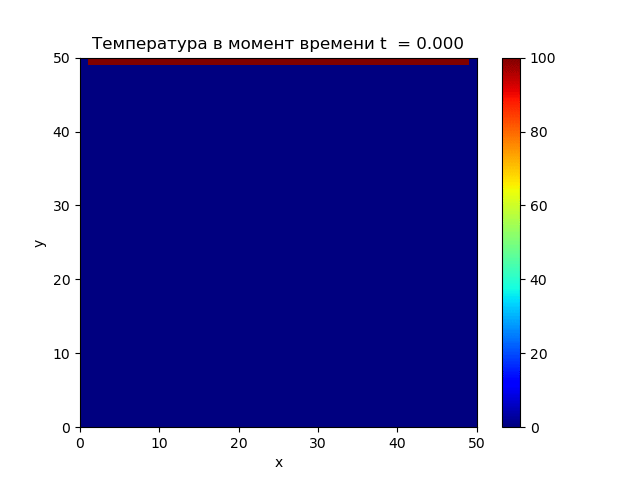
\includegraphics[width=\textwidth]{hes_pic-0.png}
\end{subfigure}
\hfill
\begin{subfigure}[b]{0.5\textwidth}
	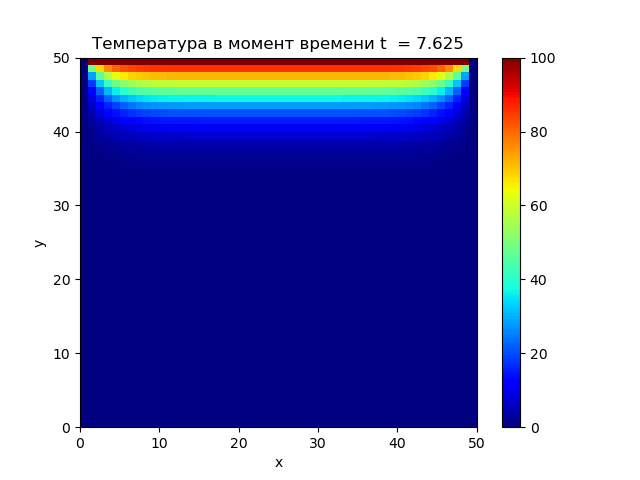
\includegraphics[width=\textwidth]{hes_pic-61.png}
\end{subfigure}

\begin{subfigure}[b]{0.5\textwidth}
	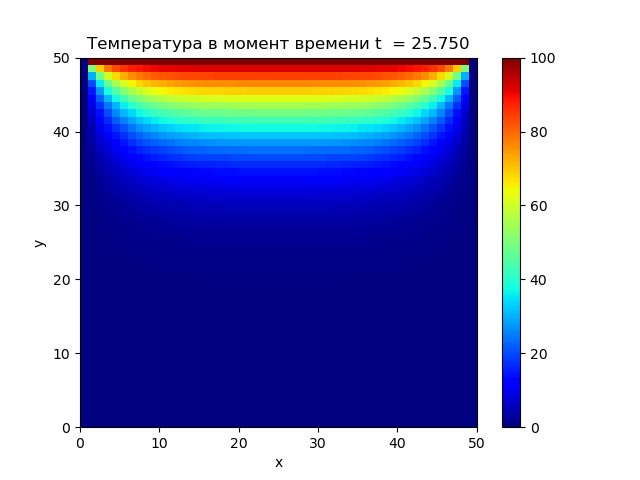
\includegraphics[width=\textwidth]{hes_pic-206.png}
\end{subfigure}
\hfill
\begin{subfigure}[b]{0.5\textwidth}
	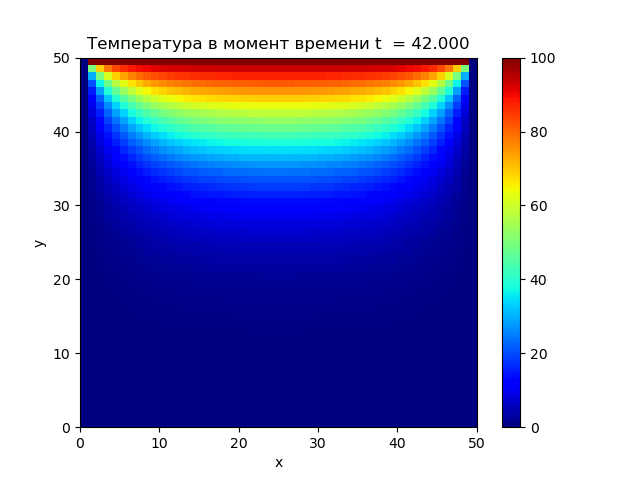
\includegraphics[width=\textwidth]{hes_pic-336.png}
\end{subfigure}

\begin{subfigure}[b]{0.5\textwidth}
	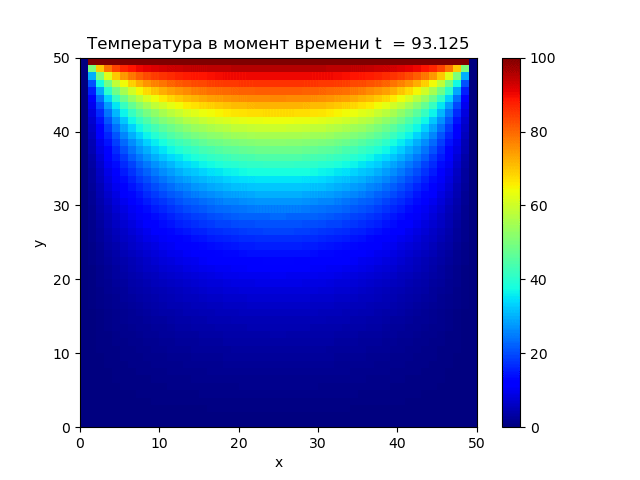
\includegraphics[width=\textwidth]{hes_pic-745.png}
\end{subfigure}
\hfill
\begin{subfigure}[b]{0.5\textwidth}
	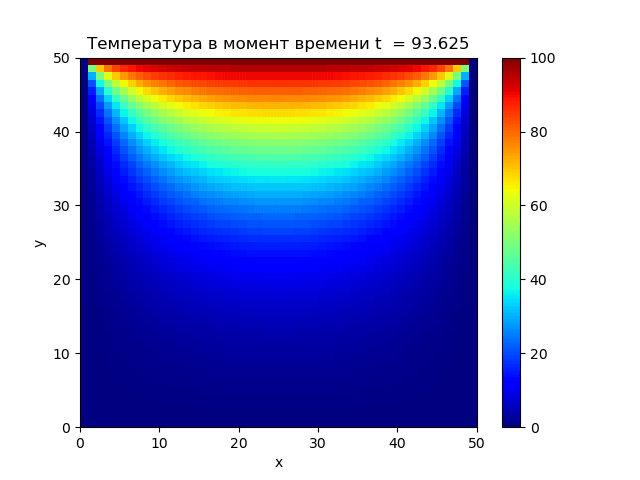
\includegraphics[width=\textwidth]{hes_pic-749.png}
\end{subfigure}
\captionsetup{labelfont=bf, labelsep=space}
\caption{Графическое отображение решения в момент времени $t$}
\end{figure}

В качестве тела для нагрева была взята тонкая квадратная пластина со стороной в 50 единиц длины. Температура внутри пластины ровна 0 (в момент времени $t=0$). Для данной модели были также взяты $h = 1$ и $\kappa = 2.0$

\newpage

\section*{Заключение}
\addcontentsline{toc}{section}{Заключение}
В данной работе был продемонстрирован один из методов развёртывания вычислительного кластера.
В ходе работы была полностью решена проблема автоматизации процесса развёртывания c возможностью дальнейшего масштабирования, разработана документация для облегчения дальнейшего обслуживания, а  также ряд инструментов облегчающих выполнение задач администрирования в будущем.  Был произведён сравнительный анализ результатов тестирования и показан один из способов решения уравнения теплопроводности. Кластер был запущен в эксплуатацию и используется сотрудниками Ярославского государственного университета.

\newpage

\addcontentsline{toc}{section}{Список литературы}
\fontsize{12}{12}\selectfont

\begin{thebibliography}{99}
\bibitem{top500}
Erich Strohmaier Jack Dongarra Horst Simon Martin Meuer, The TOP500 project,
URL: https://www.top500.org/lists/ (дата обращения: 29.04.21)


\bibitem{slurm-pmix} 
Artem Y. Polyakov, Joshua S. Ladd, Boris I. Karasev, Slurm PMIx support,
URL: https://slurm.schedmd.com/SC17/Mellanox\_Slurm\_pmix\_UCX\_backend\_v4.pdf (дата обращения: 27.04.21)

\bibitem{slurm-mpi} 
Morris Jette, Artem Y. Polyakov,  Tim Wickberg. MPI and UPC Users Guide,
URL: https://slurm.schedmd.com/mpi\_guide.html (дата обращения: 27.04.21)

\bibitem{mpi-over-ib}
Gil Bloch, MPI over InfiniBand,
URL: https://www.open-mpi.org/papers/workshop-2006/thu\_01\_mpi\_on\_infiniband.pdf (дата обращения: 28.04.21)

\bibitem{intel-ib}
Виктор Гурылев, Infiniband: матрица для данных,
URL: https://habr.com/ru/company/intel/blog/154339 (дата обращения: 28.04.21)

\bibitem{mpisingularity} 
Felip Moll,  Tim Wickberg. Singularity and MPI applications,
URL: https://sylabs.io/guides/3.3/user-guide/mpi.html (дата обращения: 27.04.21)

\bibitem{hier}
Rusty Russell, Daniel Quinlan, Linux Foundation inc.. Filesystem Hierarchy Standard [2004 --- ],
URL: https://refspecs.linuxfoundation.org/FHS\_3.0/fhs-3.0.pdf (дата обращения 17.05.21)

\bibitem{mitkerberos}
MIT Kerberos Consortium, MIT Kerberos Documentation/keytab,
URL: https://web.mit.edu/kerberos/krb5-devel/doc/basic/keytab\_def.html (дата обращения 20.05.21)

\bibitem{linpack}
Jack J. Dongarra, Piotr Luszczek, Antoine Petitet, The LINPACK Benchmark: Past, Present, and Future / 2002 ,
URL: http://www.netlib.org/utk/people/JackDongarra/PAPERS/hplpaper.pdf (дата обращения 25.05.21)

\bibitem{ftcs}
Gerald Recktenwald. FTCS Solution to  the Heat Equation,
URL: http://web.cecs.pdx.edu/~gerry/class/ME448/lecture/pdf/FTCS\_slides.pdf (дата
обращения 23.05.21)

\bibitem{mpidoc}
The OpenMPI Project, Open MPI v4.1.1 documentation,
URL: https://www.open-mpi.org/doc/v4.1 (дата обращения 23.05.21)
\end{thebibliography}

\newpage

\begin{flushright}Приложение А\end{flushright}
\centerline{\textbf{Скрипт сборки пакетов}}
\addcontentsline{toc}{section}{Приложение А --- Скрипт сборки пакетов}

\begin{minted}[breaklines,linenos,fontsize=\footnotesize]{shell}
#!/usr/bin/env bash

# The script accepts a directory
# with needed tarballs as an argument
# so make sure that you put everything you need there
# before running the script.
# Do not also forget to track down
# the $mpi3_prefix and $mpi4_prefix on OpenMPI version changes

if [[ ${UID} -ne 0 ]]; then
    echo "You must be logged in as root to run this script!"
    exit 1
fi

# temporary directory for deb files

mkdir -p /tmp/deb_packages

# shut up perl nagging
export LC_ALL=C
export LANGUAGE=C

# shut up slurm mysql nagging

export HAVEMYSQLCONFIG=/usr/bin/mysql_config
export ac_have_mysql=yes

apt-get install -y  libkrb5-dev bison \
  libevent-dev munge libmunge-dev flex libssl-dev uuid-dev \
        checkinstall m4 libnuma-dev gcc-multilib gfortran > /dev/null 2>&1

tempdir=$(mktemp -d /tmp/slurm-build-XXX --suffix=-$(date +"%m-%d-%y"))

basic_prefix="/usr/local"
mpi4_prefix="/usr/mpi/gcc/openmpi-4.0.1"
mpi3_prefix="/usr/mpi/gcc/openmpi-3.1.3"
mpi1_prefix="/usr/mpi/gcc/openmpi-1.6.5-32"
toolchain_prefix="/usr/local/autotools"

if [[ -z "$1" ]]; then
    echo "Ooops... you seem to forget to point a dir!"
    exit 1
fi

run_binary_build() {
    make -j$(nproc)
    checkinstall -y --pakdir=/tmp/deb_packages --install=no \
    --pkgname=$1 --pkgversion=$2
}

# The run_binary_build() function
# accepts two optional arguments
# that can be used when we need
# few versions of the same package
# installed at the same time
# or neither versior nor name of
# a package is not clear for checkinstall
# look at either singularity or hwloc or openmpi examples

run_source_build() {
        make -j$(nproc)
        make install

}

# The run_source_build() function is only needed for
# packages that we do not want/need to convert to
# the binary packages but need them to build
# binaries (libtool/autoconf/automake/m4 and so on)

cd $1

for item in *tar*; do
    tar xf ${item} -C ${tempdir}
done

# install cuda repositories
dpkg -i --force-overwrite cuda-repo-ubuntu1604-8-0-local-ga2_8.0.61-1_amd64.deb
dpkg -i --force-overwrite cuda-repo-ubuntu1804-10-2-local-10.2.89-440.33.01_1.0-1_amd64.deb

apt-key add /var/cuda-repo-10-2-local-10.2.89-440.33.01/7fa2af80.pub
apt-key add /var/cuda-repo-8-0-local-ga2/7fa2af80.pub

apt-get update

cd ${tempdir}

files=( hwloc-1*
        hwloc-2*
        libevent*
        m4*
        autoconf*
        automake*
        libtool*
        pmix*
        slurm*
        auks*
        openmpi-1*
        openmpi-3*
        openmpi-4*
        go*
        singularity* )

echo "Just make sure that you have right packages to install"

echo ${files[@]}

read -n 1 -s -r -p "And then press any key to continue "

# copy go properly
mv -f ${tempdir}/go ${basic_prefix}/

# hwloc-1
if [[ -e "${files[0]}" ]]; then
        pushd "${files[0]}"
       ./configure --prefix="${basic_prefix}/hwloc-1" && run_binary_build "hwloc1" && popd
fi

# hwloc-2
if [[ -e  "${files[1]}" ]]; then
        pushd "${files[1]}"
        ./configure --prefix="${basic_prefix}/hwloc-2" && run_binary_build "hwloc2" && popd
fi

# libevent
if [[ -e "${files[2]}"  ]]; then
        pushd "${files[2]}"
       ./configure --prefix="${basic_prefix}/libevent" && run_binary_build "libevent" "2.1.10" &&  popd
fi

export PATH=${PATH}:/usr/local/autotools/bin

# m4
if [[ -e "${files[3]}"  ]]; then
        pushd "${files[3]}"
       ./configure --prefix=${toolchain_prefix} && run_source_build && popd
fi

# autoconf
if [[ -e "${files[4]}"  ]]; then
        pushd "${files[4]}"
       ./configure --prefix=${toolchain_prefix} && run_source_build && popd

fi

# automake
if [[ -e "${files[5]}"  ]]; then
        pushd "${files[5]}"
       ./configure --prefix=${toolchain_prefix} && run_source_build && popd
fi

# libtool
if [[ -e "${files[6]}"  ]]; then
        pushd "${files[6]}"
       ./configure --prefix=${toolchain_prefix} && run_source_build && popd
fi

# pmix
if [[ -e "${files[7]}" ]]; then
        pushd "${files[7]}"
        ./autogen.pl
        ./configure --prefix="${basic_prefix}/pmix" --with-platform=optimized --with-libevent=/usr/local/libevent --disable-pmi-backward-compatibility \
         && run_binary_build "pmix" "3.1.4" && popd
fi

# slurm
if [[ -e "${files[8]}" ]]; then
        pushd "${files[8]}"
        ./configure --prefix="${basic_prefix}/slurm" --sysconfdir=/etc/slurm --without-ucx --without-freeipmi --with-pmix="${basic_prefix}/pmix" \
        --with-mysql_config=/usr/bin \
         && run_binary_build && popd
fi

# auks
if [[ -e "${files[9]}" ]]; then
        pushd "${files[9]}"
        # temporary hack, makefiles may be changed in the future
        sed -i 's/-lkrb5 -pthread/-lkrb5 -lpthread/g' src/api/auks/Makefile.am
        sed -i 's/-lkrb5 -pthread/-lkrb5 -lpthread/g' src/api/auks/Makefile.in
        sed -i 's/MANS = $(man1_MANS) $(man5_MANS) $(man8_MANS)/MANS = $(man1_MANS) $(man5_MANS)/g' doc/man/Makefile.in
        sed -i 's/install-man: install-man1 install-man5 install-man8/install-man: install-man1 install-man5/g' doc/man/Makefile.in
        ./configure --prefix="${basic_prefix}/auks" --sysconfdir=/etc/auks --with-slurm="${basic_prefix}/slurm" \
        && run_binary_build && popd
fi


# install cuda
apt-get --reinstall install -y cuda-8-0
apt-get --reinstall install -y cuda


# openmpi-1
if [[ ! -d "${file[10]}" ]]; then
        pushd "${files[10]}"
        ./configure --prefix=${mpi1_prefix} \
        --disable-vt \
        --build=i686-pc-linux-gnu \
        --with-slurm="${basic_prefix}/slurm" \
        && run_binary_build "openmpi1" && popd
fi

# openmpi-3 and openmpi-4 with cuda
if [[ -e "${files[11]}" ]]; then
        pushd "${files[11]}"
        ./configure --prefix=${mpi3_prefix} \
        --with-slurm="${basic_prefix}/slurm" \
        --with-libevent="${basic_prefix}/libevent" \
        --with-hwloc="${basic_prefix}/hwloc-1" \
        --with-pmix="${basic_prefix}/pmix" \
        --with-cuda=/usr/local/cuda \
        --without-ucx \
         && run_binary_build "openmpi3" && popd
fi

if  [[ -e "${files[12]}" ]]; then
        pushd "${files[12]}"
        ./configure --prefix=${mpi4_prefix} \
        --with-slurm=${basic_prefix} \
        --with-libevent="${basic_prefix}/libevent" \
        --with-hwloc="${basic_prefix}/hwloc-2" \
        --with-pmix="${basic_prefix}/pmix" \
        --with-cuda=/usr/local/cuda \
        --without-ucx \
        && run_binary_build "openmpi4" && popd
fi

# openmpi-3 and openmpi-4 without cuda
if [[ -e "${files[11]}" ]]; then
        pushd "${files[11]}"
        ./configure --prefix="${mpi3_prefix}_without_cuda" \
        --with-slurm="${basic_prefix}/slurm" \
        --with-libevent="${basic_prefix}/libevent" \
        --with-hwloc="${basic_prefix}/hwloc-1" \
        --with-pmix="${basic_prefix}/pmix" \
        --without-cuda \
        --without-ucx \
         && run_binary_build "openmpi3_without_cuda" && popd
fi

if  [[ -e "${files[12]}" ]]; then
        pushd "${files[12]}"
        ./configure --prefix="${mpi4_prefix}_without_cuda" \
        --with-slurm="${basic_prefix}/slurm" \
        --with-libevent="${basic_prefix}/libevent" \
        --with-hwloc="${basic_prefix}/hwloc-2" \
        --with-pmix="${basic_prefix}/pmix" \
        --without-cuda \
        --without-ucx \
        && run_binary_build "openmpi4_without_cuda" && popd
fi

export PATH=${basic_prefix}/go/bin:${PATH}:${GOPATH}/bin

# singularity
if [[ -e "${files[14]}" ]]; then
       pushd "${files[14]}"
       ./mconfig --prefix=/usr/local/singularity && \
       cd ./builddir && run_binary_build "singularity" "3.5.3" && popd
fi

chmod 4755 ${basic_prefix}/singularity/libexec/singularity/bin/starter-suid


mkdir -p /tmp/clusterbuild

mv -f ${basic_prefix}/* /tmp/clusterbuild > /dev/null 2>&1
# we install cuda per node using saltstack
rm -fr /tmp/clusterbuild/cuda*
rm -fr /var/cuda*
rm -fr /tmp/clusterbuild/autotools
rm -fr  /etc/apt/sources.list.d/*cuda*

echo "---------------------------------------------------"
echo "compilation finished!"
echo "BINARY packages here: (add them to the repository)"
echo "/tmp/deb_packages"
echo "----------------------------------------------------"

rm -fr ${tempdir}

apt-get remove -y --purge cuda* > /dev/null 2>&1
\end{minted}

\newpage

\begin{flushright}Приложение 	Б\end{flushright}
\centerline{\textbf{Файл конфигурации slurm}}
\addcontentsline{toc}{section}{Приложение Б --- Файл конфигурации slurm}

\begin{minted}[linenos,tabsize=2,breaklines,fontsize=\footnotesize]{text}
SlurmctldHost=control1
DisableRootJobs=YES
MpiDefault=pmix_v3
PluginDir=/usr/local/slurm/lib/slurm
PlugStackConfig=/etc/slurm/plugstack.conf
ProctrackType=proctrack/linuxproc
ReturnToService=1
SlurmctldPidFile=/var/run/slurmctld.pid
SlurmctldPort=6817
SlurmdPidFile=/var/run/slurmd.pid
SlurmdPort=6818
SlurmdSpoolDir=/home/slurm/slurmd
SlurmUser=slurm
StateSaveLocation=/home/slurm
SwitchType=switch/none
TaskPlugin=task/affinity
TaskPluginParam=Sched
InactiveLimit=0
KillWait=30
MinJobAge=300
SlurmctldTimeout=120
SlurmdTimeout=300
Waittime=0
FastSchedule=1
SchedulerType=sched/builtin
SelectType=select/cons_res
SelectTypeParameters=CR_Core
AccountingStorageEnforce=limits
AccountingStoragePort=7031
AccountingStorageType=accounting_storage/slurmdbd
AccountingStoreJobComment=YES
ClusterName=cluster
JobCompType=jobcomp/none
JobContainerType=job_container/none
JobAcctGatherFrequency=30
JobAcctGatherType=jobacct_gather/none
SlurmctldDebug=debug5
SlurmctldLogFile=/tmp/slurmctld.log
SlurmdDebug=debug5
SlurmdLogFile=/tmp/slurmd.log
NodeName=dnode[01,02,03,04] RealMemory=64000 Sockets=2 CoresPerSocket=10 ThreadsPerCore=1 State=UNKNOWN
NodeName=dnode[05,06,07,08] RealMemory=128000 Sockets=2 CoresPerSocket=10 ThreadsPerCore=1 State=UNKNOWN
NodeName=dnode[09,10,11,12,13,14] RealMemory=16000 Sockets=2 CoresPerSocket=6 ThreadsPerCore=1 State=UNKNOWN
NodeName=cnode[1,2,3,4,5,6,7] RealMemory=64000 Sockets=2 CoresPerSocket=8 ThreadsPerCore=1 State=UNKNOWN
PartitionName=all Nodes=cnode[1,2,3,4,5,6,7],dnode[01,02,03,04,05,06,07,08,09,10,11,12,13,14] MaxTime=INFINITE State=UP
PartitionName=uni Nodes=cnode[1,2,3,4,5,6,7] MaxTime=INFINITE State=UP
\end{minted}

\newpage

\begin{flushright}Приложение В\end{flushright}
\centerline{\textbf{Файл конфигурации slurmdbd}}
\addcontentsline{toc}{section}{Приложение В --- Файл конфигурации slurmdbd}

\begin{minted}[linenos,tabsize=2,breaklines]{text}
AuthType=auth/munge
AuthInfo=/var/run/munge/munge.socket.2
StorageType=accounting_storage/mysql
DbdAddr=localhost
DbdPort=7031
DbdHost=localhost
MessageTimeout=15
DebugLevel=verbose
DefaultQOS=normal,standby
LogFile=/tmp/slurmdbd.log
PidFile=/var/run/slurmdbd.pid
StorageHost=localhost
StoragePort=3306
StoragePass=x4qGD*KNHDb9-Bu>u8N{
StorageUser=slurm
StorageLoc=slurm_acct_db
SlurmUser=slurm
\end{minted}

\newpage

\begin{flushright}Приложение Г\end{flushright}
\centerline{\textbf{Скрипт синхронизации с ldap}}
\addcontentsline{toc}{section}{Приложение Г --- Скрипт синхронизации с ldap}

\begin{minted}[breaklines,linenos,fontsize=\footnotesize]{python}
#!/usr/bin/env  python3

from ldap3 import Server, Connection, ALL
from subprocess import run
import sys


def main():
    server = Server(
                    'network1.int.accelcomp.org',
                    get_info=ALL)

    conn = Connection(
        server,
        auto_bind=True)

    conn.search(
        search_base='ou=groups,dc=int,dc=accelcomp,dc=org',
        search_filter='(|(gidNumber=5001)(gidNumber=5002)(gidNumber=5003))',
        paged_size=100,
        attributes=['*']
    )

    groups_handler = conn.entries

    conn.search(
        search_base='ou=people,dc=int,dc=accelcomp,dc=org',
        search_filter='(objectClass=inetOrgPerson)',
        paged_size=100,
        attributes=['*']
    )

    regular_users = conn.entries

    if len(sys.argv) == 2:

        # initialize cluster with a given name
        # if it did not exist before

        run("sacctmgr -i add cluster {}".format(sys.argv[1]), shell=True)
        run("sacctmgr -i add account regular", shell=True)
        run("sacctmgr -i add account power", shell=True)
        run("sacctmgr -i  add qos short_term MaxWall=10:00", shell=True)

    # just cleanup everything on each call

    run("sacctmgr -i remove User where DefaultAccount=regular", shell=True)

    # add accounts and give permissions (parse groups)

    for uni_member in groups_handler[1].memberUid:
        run("sacctmgr -i add user {} DefaultAccount=regular Partition=uni".format(uni_member), shell=True)
        run("sacctmgr -i modify user where name={} account=regular set qos+=short_term defaultqos=short_term"
            .format(uni_member), shell=True)

    for acc_member in groups_handler[2].memberUid:
        run("sacctmgr -i add user {} DefaultAccount=regular".format(acc_member), shell=True)
        run("sacctmgr -i modify user where name={} account=regular set qos+=short_term defaultqos=short_term"
            .format(acc_member), shell=True)

    # parse all ldap users

    for user in regular_users:
        run("sacctmgr -i add user {} DefaultAccount=regular Partition=debug".format(user.uid), shell=True)
        run("sacctmgr -i modify user where name={} account=regular set qos+=short_term defaultqos=short_term"
            .format(user.uid), shell=True)

    for power_member in groups_handler[0].memberUid:
        run("sacctmgr -i add user {} DefaultAccount=power".format(power_member), shell=True)
        run("sacctmgr -i modify user where name={} account=power set defaultqos=normal"
            .format(power_member), shell=True)


if __name__ == "__main__":
    main()
\end{minted}

\newpage

\begin{flushright}Приложение Д\end{flushright}
\centerline{\textbf{Файл конфигурации HPL.dat}}
\addcontentsline{toc}{section}{Приложение Д --- Файл конфигурации HPL.dat}
\begin{minted}[linenos,tabsize=2,breaklines]{text}
HPLinpack benchmark input file
Innovative Computing Laboratory, University of Tennessee
HPL.out      output file name (if any) 
6            device out (6=stdout,7=stderr,file)
1            # of problems sizes (N)
115584         Ns
1            # of NBs
192           NBs
0            PMAP process mapping (0=Row-,1=Column-major)
1            # of process grids (P x Q)
4            Ps
4            Qs
16.0         threshold
1            # of panel fact
2            PFACTs (0=left, 1=Crout, 2=Right)
1            # of recursive stopping criterium
4            NBMINs (>= 1)
1            # of panels in recursion
2            NDIVs
1            # of recursive panel fact.
1            RFACTs (0=left, 1=Crout, 2=Right)
1            # of broadcast
1            BCASTs (0=1rg,1=1rM,2=2rg,3=2rM,4=Lng,5=LnM)
1            # of lookahead depth
1            DEPTHs (>=0)
2            SWAP (0=bin-exch,1=long,2=mix)
64           swapping threshold
0            L1 in (0=transposed,1=no-transposed) form
0            U  in (0=transposed,1=no-transposed) form
1            Equilibration (0=no,1=yes)
8            memory alignment in double (> 0)
##### This line (no. 32) is ignored (it serves as a separator). ######
0                               Number of additional problem sizes for PTRANS
1200 10000 30000                values of N
0                               number of additional blocking sizes for PTRANS
40 9 8 13 13 20 16 32 64        values of NB
\end{minted}

\newpage

\begin{flushright}Приложение Е\end{flushright}
\centerline{\textbf{MPI реализация рекурсивной формулы}}
\addcontentsline{toc}{section}{Приложение Е --- MPI реализация рекурсивной формулы}
\begin{minted}{C}
	// явно задаем переменные для вычисления
	diagx = -2.0 + hx*hx/(2*k0*dt);
	diagy = -2.0 + hy*hy/(2*k0*dt);
	weightx = k0 * dt/(hx*hx);
	weighty = k0 * dt/(hy*hy);
	
	// Обновляем значение подобластей в сетке
	for (i=xs[me];i<=xe[me];i++)
	for (j=ys[me];j<=ye[me];j++)
	x[i][j] = weightx*(x0[i-1][j] + x0[i+1][j] + x0[i][j]*diagx)
	+ weighty*(x0[i][j-1] + x0[i][j+1] + x0[i][j]*diagy)
	
\end{minted}

\newpage

\begin{flushright}Приложение Ж\end{flushright}
\centerline{\textbf{Функция межпроцессорного взаимодействия}}
\addcontentsline{toc}{section}{Приложение Ж --- Функция межпроцессорного взаимодействия }
\begin{minted}{C}
while (!converge) {
	// увеличиывем шаг и время
	t = t + dt;
	step = step + 1;
	// Прогоганяем FTCS схему ровно один раз
	computeNext(x0, x, dt, hx, hy, &localDiff, me, xsi, ysi, xei, yei, k0);
	updateBound(x0, neighBor, comm2d, column_type, ime, xsi, ysi, xei, yei, ycell);
	MPI_Allreduce(&localDiff, &result, 1, MPI_DOUBLE, MPI_SUM, comm);
	result = sqrt(result);
	// Выходим из цыкла если считать уже нечего
	if ((result < epsilon) || (step > maxStep)) break;
}

\end{minted}
%
%
%
\end{document}
